\documentclass[11pt]{article}
\usepackage[margin=1in]{geometry}
\usepackage{graphicx}
\usepackage{booktabs}
\usepackage{float}
\usepackage{hyperref}
\usepackage{longtable}
\usepackage{array}
\usepackage{caption}
\title{SEDS 537 Machine Learning Take-Home Midterm}
\author{Alperen Ertan \\ 313011004}
\date{Prepared on \today}

\begin{document}
\maketitle

\section*{Reproducibility}
All experiments use a fixed random seed of 42. The codebase is structured to run end-to-end with a single command:
\texttt{jupyter notebook notebook/midterm.ipynb}.

\noindent \textbf{Repository link:} \url{https://github.com/alperen8/SEDS537_Midterm}

\section{Question 1: Regression on California Housing}
The California Housing dataset contains 20640 observations. Three regression families were compared: Linear Regression, Ridge Regression, and Random Forest Regressor. I evaluated baseline models, scaled variants, and degree-2 polynomial variants on the same train/test split.

\begin{table}[H]
\centering
\begin{tabular}{lllll}
\toprule
experiment & model & RMSE & MAE & R2 \\
\midrule
baseline & Linear Regression & 0.7456 & 0.5332 & 0.5758 \\
baseline & Ridge Regression & 0.7450 & 0.5332 & 0.5764 \\
baseline & Random Forest & 0.5039 & 0.3266 & 0.8062 \\
scaled & Linear Regression & 0.7456 & 0.5332 & 0.5758 \\
scaled & Ridge Regression & 0.7455 & 0.5332 & 0.5758 \\
scaled & Random Forest & 0.5038 & 0.3265 & 0.8063 \\
polynomial\_degree\_2 & Linear Regression & 0.6814 & 0.4670 & 0.6457 \\
polynomial\_degree\_2 & Ridge Regression & 0.7478 & 0.5291 & 0.5733 \\
polynomial\_degree\_2 & Random Forest & 0.5127 & 0.3347 & 0.7994 \\
\bottomrule
\end{tabular}

\caption{Q1 regression metrics on the held-out test split.}
\end{table}

The strongest baseline model by RMSE was \textbf{Random Forest}, with RMSE=0.5039 and $R^2$=0.8062. Scaling produced almost no gain for the tree model, which is expected because tree splits are invariant to monotonic rescaling. Polynomial expansion improved the linear family more than the tree model because it explicitly introduced interaction terms.

\begin{figure}[H]
\centering

\includegraphics[width=0.8\textwidth]{figures/question1/histograms.png}
\caption{Q1 feature histograms.}
\end{figure}

\begin{figure}[H]
\centering

\includegraphics[width=0.72\textwidth]{figures/question1/correlation_matrix.png}
\caption{Q1 correlation matrix.}
\end{figure}

\begin{figure}[H]
\centering

\includegraphics[width=\textwidth]{figures/question1/scatter_plots.png}
\caption{Q1 scatter plots for representative features.}
\end{figure}

\begin{figure}[H]
\centering

\includegraphics[width=\textwidth]{figures/question1/residual_plots.png}
\caption{Q1 residual plots for baseline regressors.}
\end{figure}

\noindent Interpretability and predictive power moved in opposite directions here: Linear and Ridge Regression are easier to explain coefficient-by-coefficient, but the Random Forest captured nonlinear structure more effectively.

\section{Question 2: Imbalanced Classification}
For the imbalanced classification task, I used the OpenML Credit Card Fraud dataset and drew a stratified subset of 40000 rows to keep all comparisons reproducible and computationally tractable. The positive class rate in the working subset was 0.1725\%.

\begin{table}[H]
\centering
\begin{tabular}{rrl}
\toprule
class & count & percentage \\
\midrule
0 & 39931 & 99.8275 \\
1 & 69 & 0.1725 \\
\bottomrule
\end{tabular}

\caption{Q2 class distribution in the sampled dataset.}
\end{table}

\begin{table}[H]
\centering
\begin{tabular}{llllll}
\toprule
sampling & model & precision & recall & f1 & roc\_auc \\
\midrule
smote & Random Forest & 1.0000 & 0.7857 & 0.8800 & 0.9971 \\
smote & XGBoost & 1.0000 & 0.7857 & 0.8800 & 0.9921 \\
none & XGBoost & 1.0000 & 0.7143 & 0.8333 & 0.9719 \\
undersample & XGBoost & 0.7857 & 0.7857 & 0.7857 & 0.9720 \\
none & Random Forest & 1.0000 & 0.6429 & 0.7826 & 0.9254 \\
none & Logistic Regression & 0.8000 & 0.5714 & 0.6667 & 0.9884 \\
undersample & Random Forest & 0.5000 & 0.7857 & 0.6111 & 0.9662 \\
smote & Logistic Regression & 0.3793 & 0.7857 & 0.5116 & 0.9757 \\
undersample & Logistic Regression & 0.3030 & 0.7143 & 0.4255 & 0.9848 \\
\bottomrule
\end{tabular}

\caption{Q2 classification metrics across models and resampling strategies.}
\end{table}

The best-performing configuration by F1-score was \textbf{Random Forest} with \textbf{smote}. It achieved precision=1.0000, recall=0.7857, F1=0.8800, and ROC-AUC=0.9971. In fraud detection, false negatives are usually more costly than false positives because missed fraud transactions directly translate into financial loss, so recall deserves extra emphasis even when precision falls under aggressive resampling.

\begin{figure}[H]
\centering

\includegraphics[width=0.68\textwidth]{figures/question2/best_roc_curve.png}
\caption{ROC curve for the best Q2 configuration.}
\end{figure}

\begin{figure}[H]
\centering

\includegraphics[width=0.56\textwidth]{figures/question2/confusion_smote_random_forest.png}
\caption{Confusion matrix for the best Q2 configuration.}
\end{figure}

\section{Question 3: Dimensionality Reduction and Visualisation}
This section uses a stratified subset of 4000 MNIST digits from the original 784-dimensional feature space. PCA was applied in 2D and 50D forms, and t-SNE was evaluated at perplexities 30 and 50. For downstream classification, I compared 5-fold cross-validated k-NN accuracy on the original space, PCA-reduced 50D features, and the 2D t-SNE embedding.

\begin{table}[H]
\centering
\begin{tabular}{rl}
\toprule
component & explained\_variance\_ratio \\
\midrule
1 & 0.0979 \\
2 & 0.0730 \\
3 & 0.0618 \\
4 & 0.0548 \\
5 & 0.0500 \\
6 & 0.0433 \\
7 & 0.0320 \\
8 & 0.0293 \\
9 & 0.0272 \\
10 & 0.0243 \\
\bottomrule
\end{tabular}

\caption{Q3 explained variance ratio for the first 10 PCA components.}
\end{table}

\begin{table}[H]
\centering
\begin{tabular}{lll}
\toprule
feature\_space & cv\_accuracy\_mean & cv\_accuracy\_std \\
\midrule
PCA 50D & 0.9425 & 0.0080 \\
Original 784D & 0.9300 & 0.0072 \\
t-SNE 2D & 0.9277 & 0.0115 \\
\bottomrule
\end{tabular}

\caption{Q3 5-fold cross-validated k-NN accuracy by feature space.}
\end{table}

The best feature space for k-NN was \textbf{PCA 50D}, with mean accuracy 0.9425. The first ten PCA components together explained 0.4935 of the variance within the 50-component model. PCA preserved global structure and supported downstream classification better, while t-SNE produced clearer local clusters for visual inspection. I note one methodological caveat: t-SNE does not provide a clean out-of-sample transform, so the 2D embedding was created before cross-validation and should be interpreted mainly as an exploratory comparison rather than a strict deployable pipeline.

\begin{figure}[H]
\centering

\includegraphics[width=0.7\textwidth]{figures/question3/pca_2d.png}
\caption{Q3 PCA 2D embedding.}
\end{figure}

\begin{figure}[H]
\centering

\includegraphics[width=\textwidth]{figures/question3/tsne_2d.png}
\caption{Q3 t-SNE embeddings for perplexities 30 and 50.}
\end{figure}

\section{Question 4: Clustering}
For clustering, I used the Wholesale Customers dataset with all numeric columns standardized before fitting K-Means, Agglomerative Clustering, and DBSCAN.

\begin{table}[H]
\centering
\begin{tabular}{rlll}
\toprule
k & inertia & silhouette & dbi \\
\midrule
2 & 2599.3874 & 0.3734 & 1.2581 \\
3 & 2149.2840 & 0.3568 & 1.1736 \\
4 & 1850.9488 & 0.3444 & 1.2627 \\
5 & 1551.6677 & 0.3529 & 1.1481 \\
6 & 1313.9569 & 0.3526 & 0.9588 \\
7 & 1173.9544 & 0.3638 & 0.8470 \\
8 & 1050.9697 & 0.3631 & 0.9354 \\
9 & 979.7866 & 0.3612 & 0.9524 \\
10 & 912.5085 & 0.3310 & 0.9909 \\
\bottomrule
\end{tabular}

\caption{Q4 K-Means model selection by elbow and silhouette criteria.}
\end{table}

\begin{table}[H]
\centering
\begin{tabular}{lrrll}
\toprule
algorithm & clusters\_found & noise\_points & silhouette & davies\_bouldin \\
\midrule
DBSCAN & 2 & 48 & 0.4160 & 1.0449 \\
K-Means & 2 & 0 & 0.3734 & 1.2581 \\
Agglomerative & 2 & 0 & 0.3680 & 1.2850 \\
\bottomrule
\end{tabular}

\caption{Q4 internal clustering metrics.}
\end{table}

\begin{table}[H]
\centering
\begin{tabular}{rllllllll}
\toprule
kmeans\_cluster & Channel & Region & Fresh & Milk & Grocery & Frozen & Detergents\_Paper & Delicassen \\
\midrule
0 & 1.0300 & 2.5000 & 13556.0600 & 3313.7500 & 3948.1300 & 3656.4100 & 803.4500 & 1263.3200 \\
1 & 1.9900 & 2.6300 & 8447.6000 & 11465.3000 & 17092.7900 & 1737.2300 & 7626.8700 & 2122.1500 \\
\bottomrule
\end{tabular}

\caption{Q4 K-Means cluster profiles in original feature units.}
\end{table}

The best K-Means setting was k=2, while the strongest overall clustering score came from \textbf{DBSCAN} with silhouette=0.4160. DBSCAN was tuned with a k-distance graph and ultimately used $\varepsilon=1.4048$. In practice, DBSCAN was the most parameter-sensitive method: small changes in $\varepsilon$ affected both the number of noise points and whether dense groups were merged or split.

\begin{figure}[H]
\centering

\includegraphics[width=0.85\textwidth]{figures/question4/kmeans_selection.png}
\caption{Q4 elbow and silhouette curves for K-Means.}
\end{figure}

\begin{figure}[H]
\centering

\includegraphics[width=0.68\textwidth]{figures/question4/dbscan_k_distance.png}
\caption{Q4 DBSCAN k-distance graph.}
\end{figure}

\begin{figure}[H]
\centering

\includegraphics[width=\textwidth]{figures/question4/cluster_projection.png}
\caption{Q4 PCA projection of cluster assignments.}
\end{figure}

\section{Question 5: Neural Networks on Fashion-MNIST}
Fashion-MNIST was modeled with two neural architectures implemented in PyTorch: an MLP with two hidden layers (256 and 128 units, ReLU, dropout 0.3) and a CNN with two convolution-pooling stages. Both models used the same 80/20 train/validation split from the original training set and early stopping on validation loss. Training ran on device \texttt{mps}.

\begin{table}[H]
\centering
\begin{tabular}{lllr}
\toprule
model & accuracy & macro\_f1 & epochs\_trained \\
\midrule
CNN & 0.8970 & 0.8965 & 8 \\
MLP & 0.8708 & 0.8693 & 8 \\
\bottomrule
\end{tabular}

\caption{Q5 neural network test metrics.}
\end{table}

The stronger model was \textbf{CNN}, which achieved accuracy=0.8970 and macro-F1=0.8965. This result is consistent with the convolutional inductive bias: CNNs exploit local spatial structure and weight sharing, while MLPs flatten the image and must learn those relationships indirectly.

\begin{figure}[H]
\centering
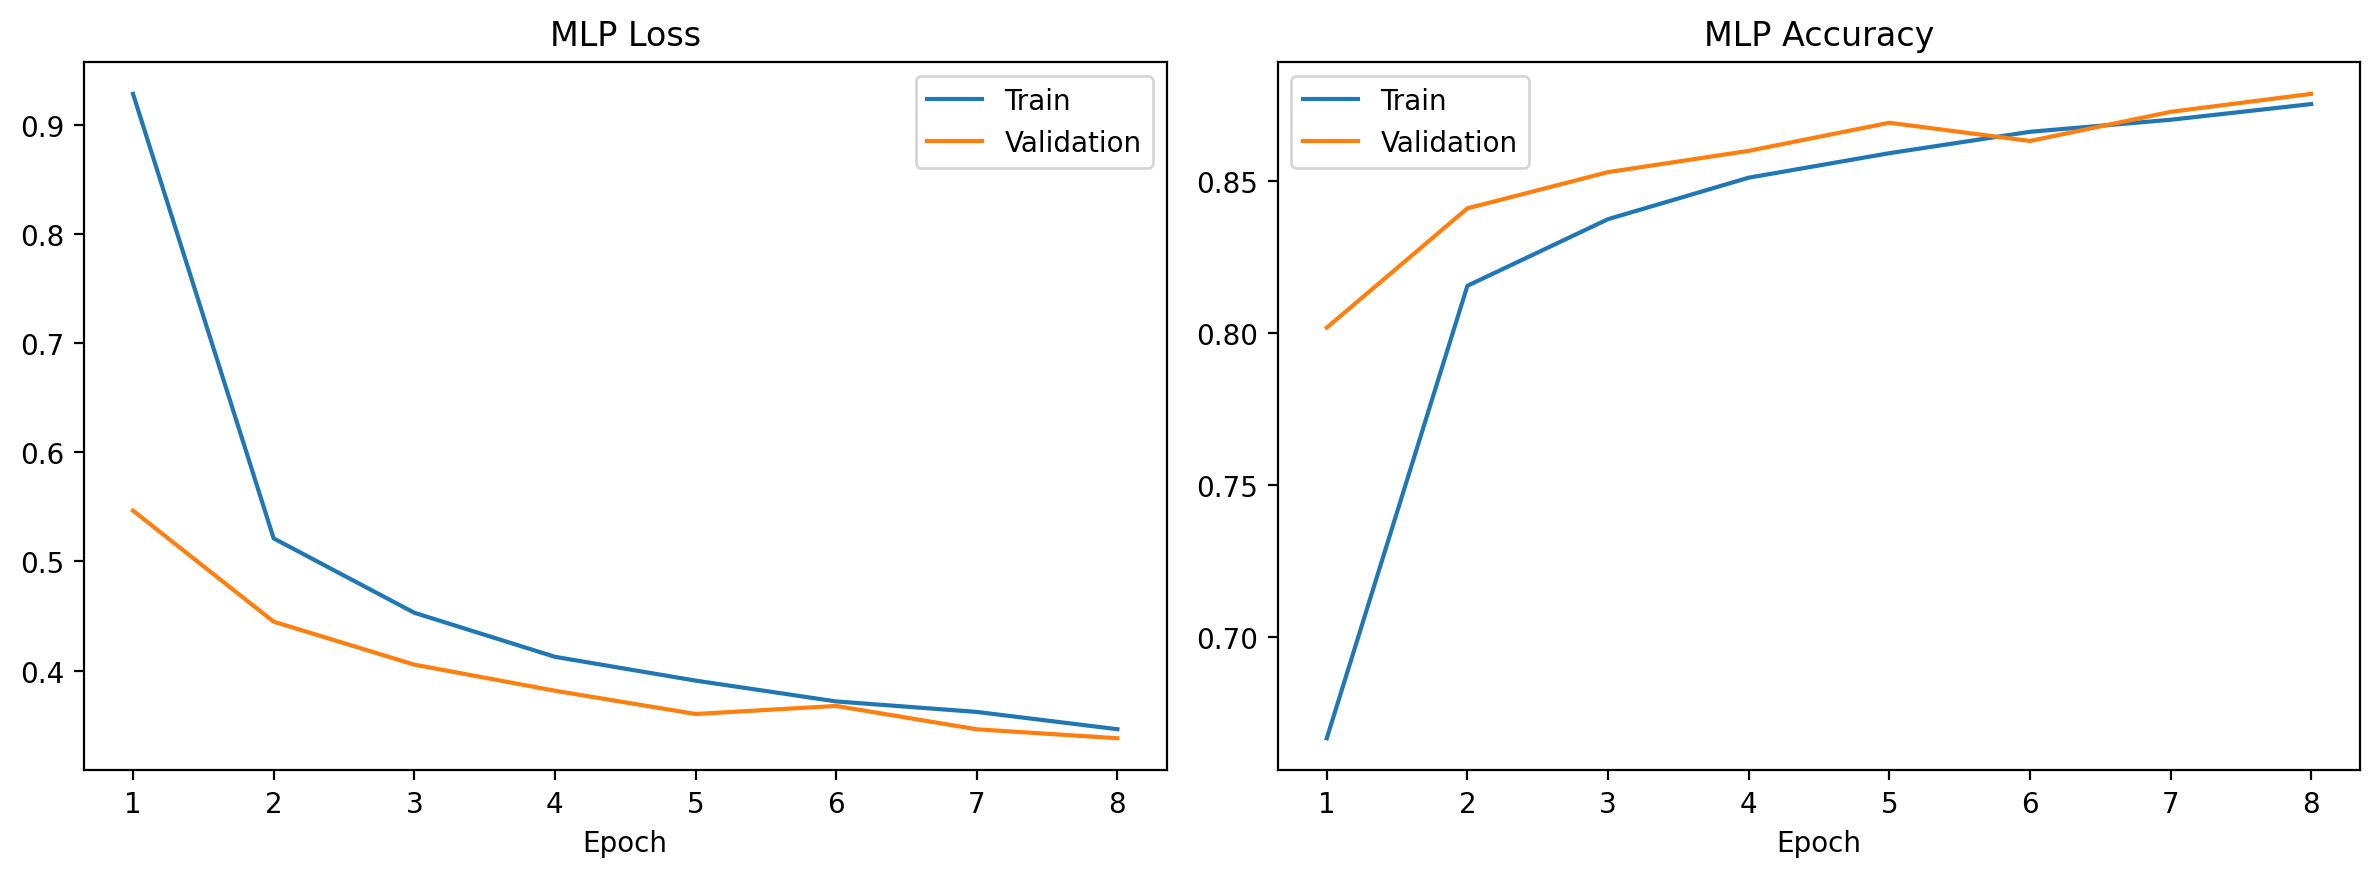
\includegraphics[width=\textwidth]{figures/question5/mlp_training_curves.png}
\caption{Q5 MLP learning curves.}
\end{figure}

\begin{figure}[H]
\centering
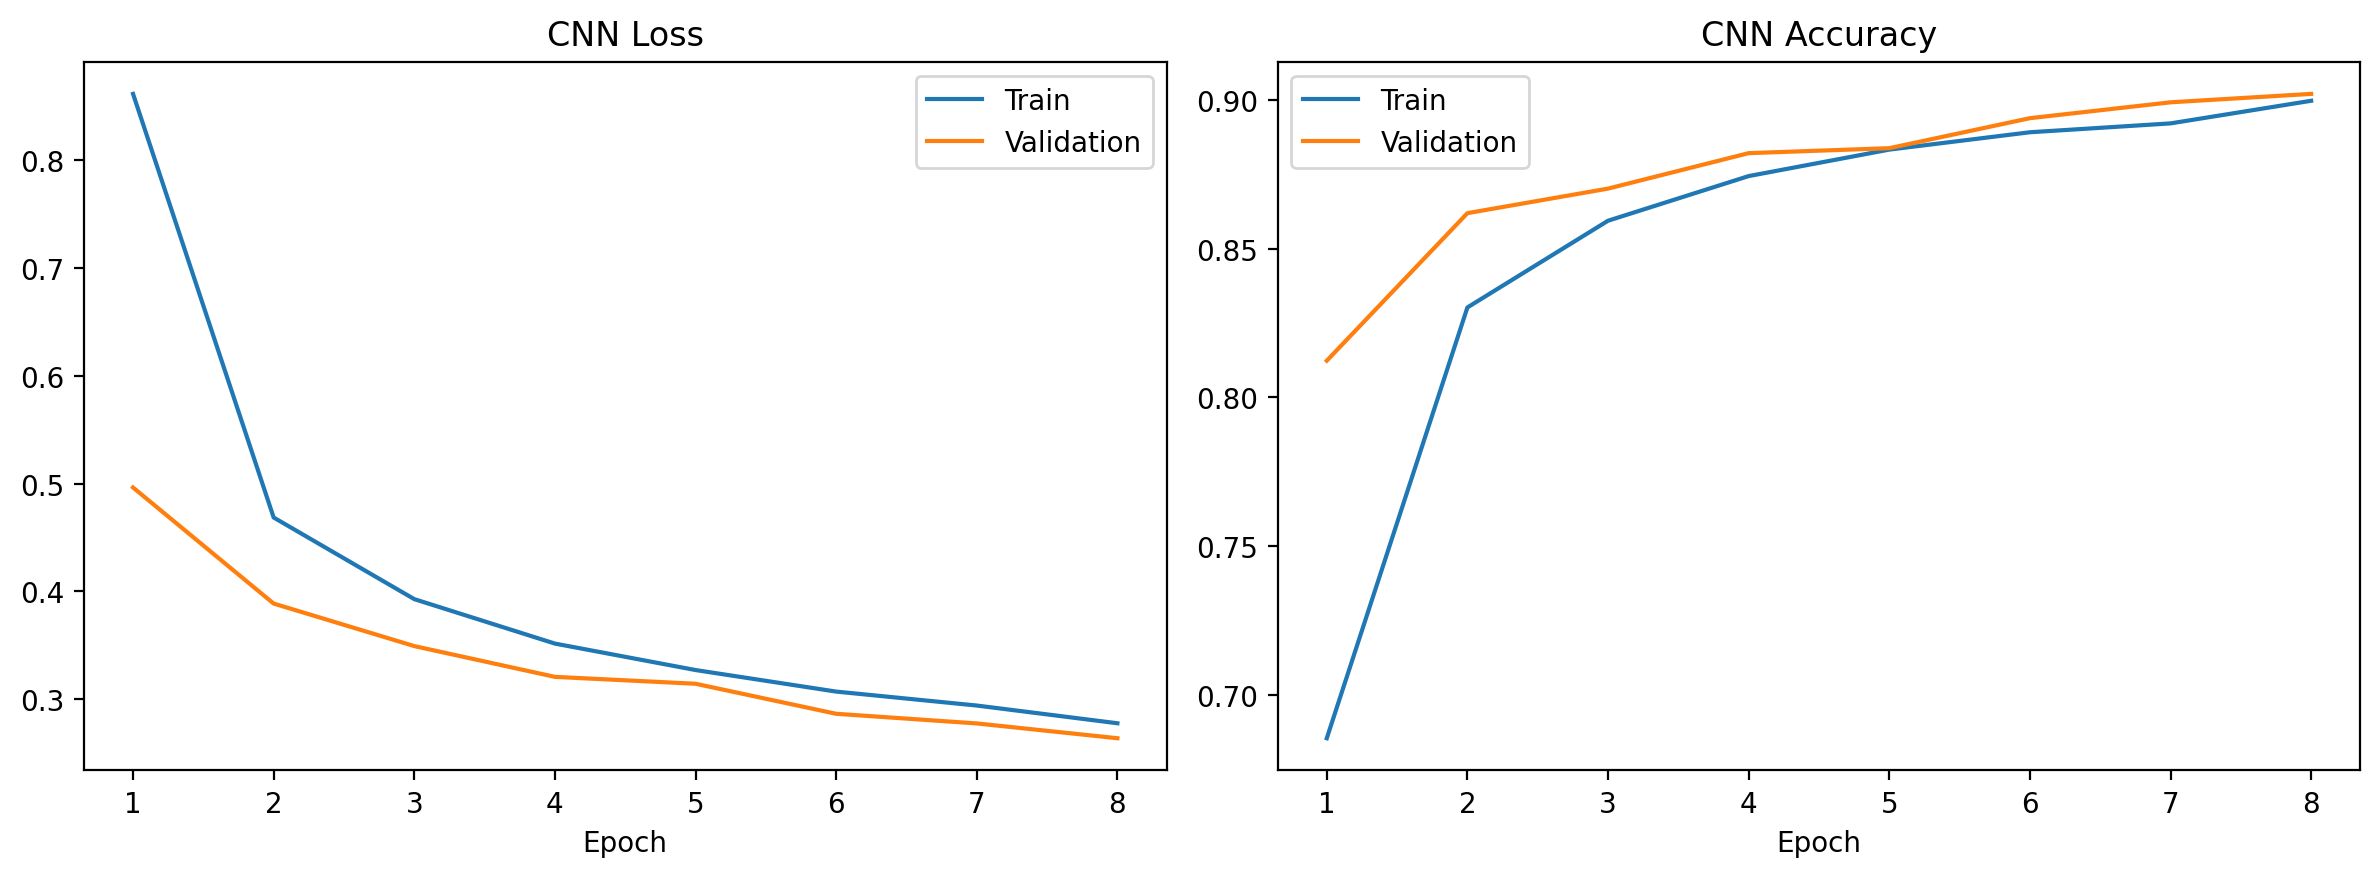
\includegraphics[width=\textwidth]{figures/question5/cnn_training_curves.png}
\caption{Q5 CNN learning curves.}
\end{figure}

\begin{figure}[H]
\centering
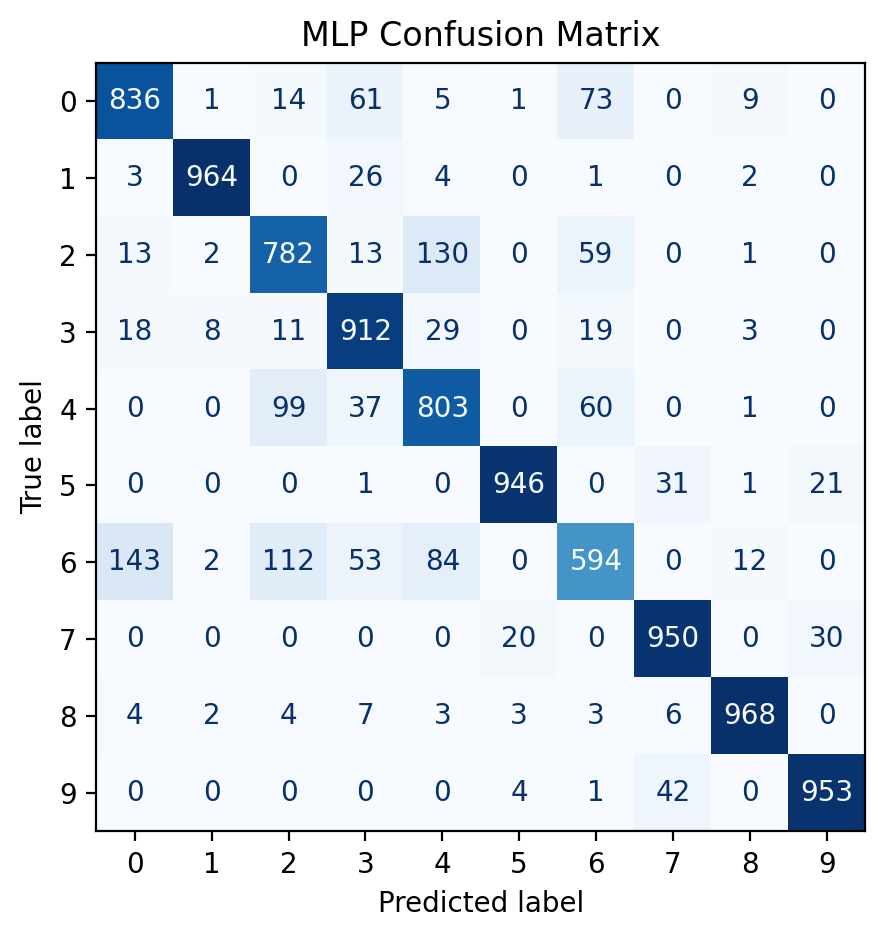
\includegraphics[width=0.7\textwidth]{figures/question5/mlp_confusion_matrix.png}
\caption{Q5 MLP confusion matrix.}
\end{figure}

\begin{figure}[H]
\centering
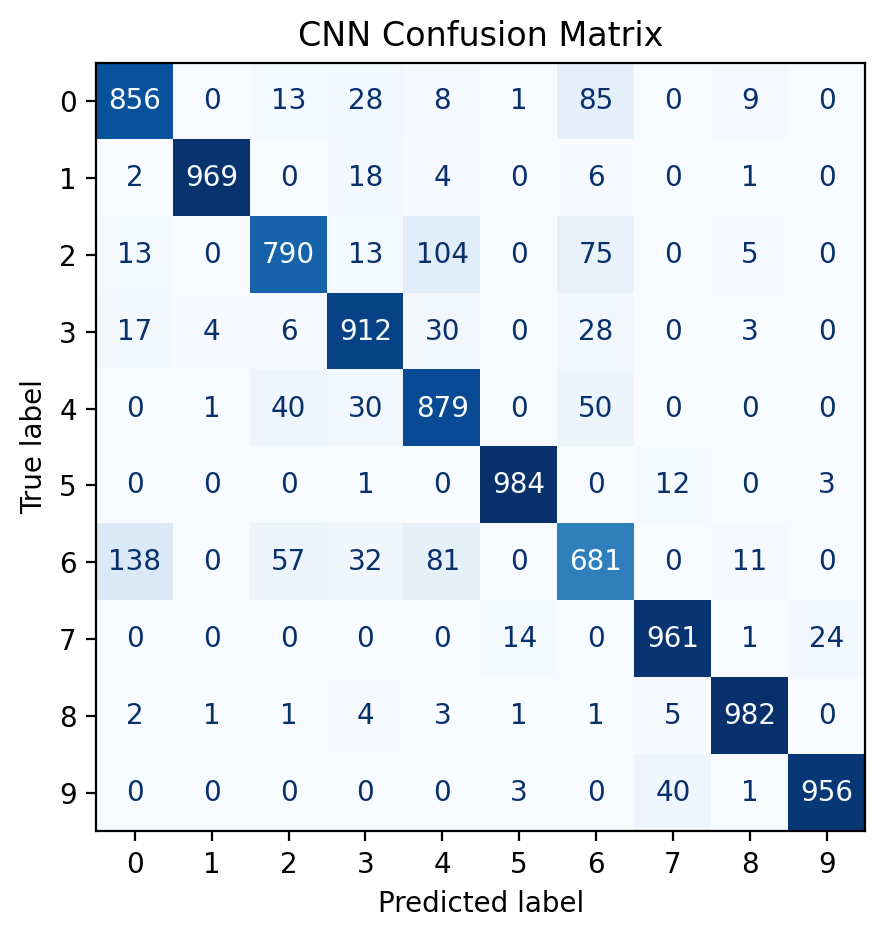
\includegraphics[width=0.7\textwidth]{figures/question5/cnn_confusion_matrix.png}
\caption{Q5 CNN confusion matrix.}
\end{figure}

\begin{figure}[H]
\centering
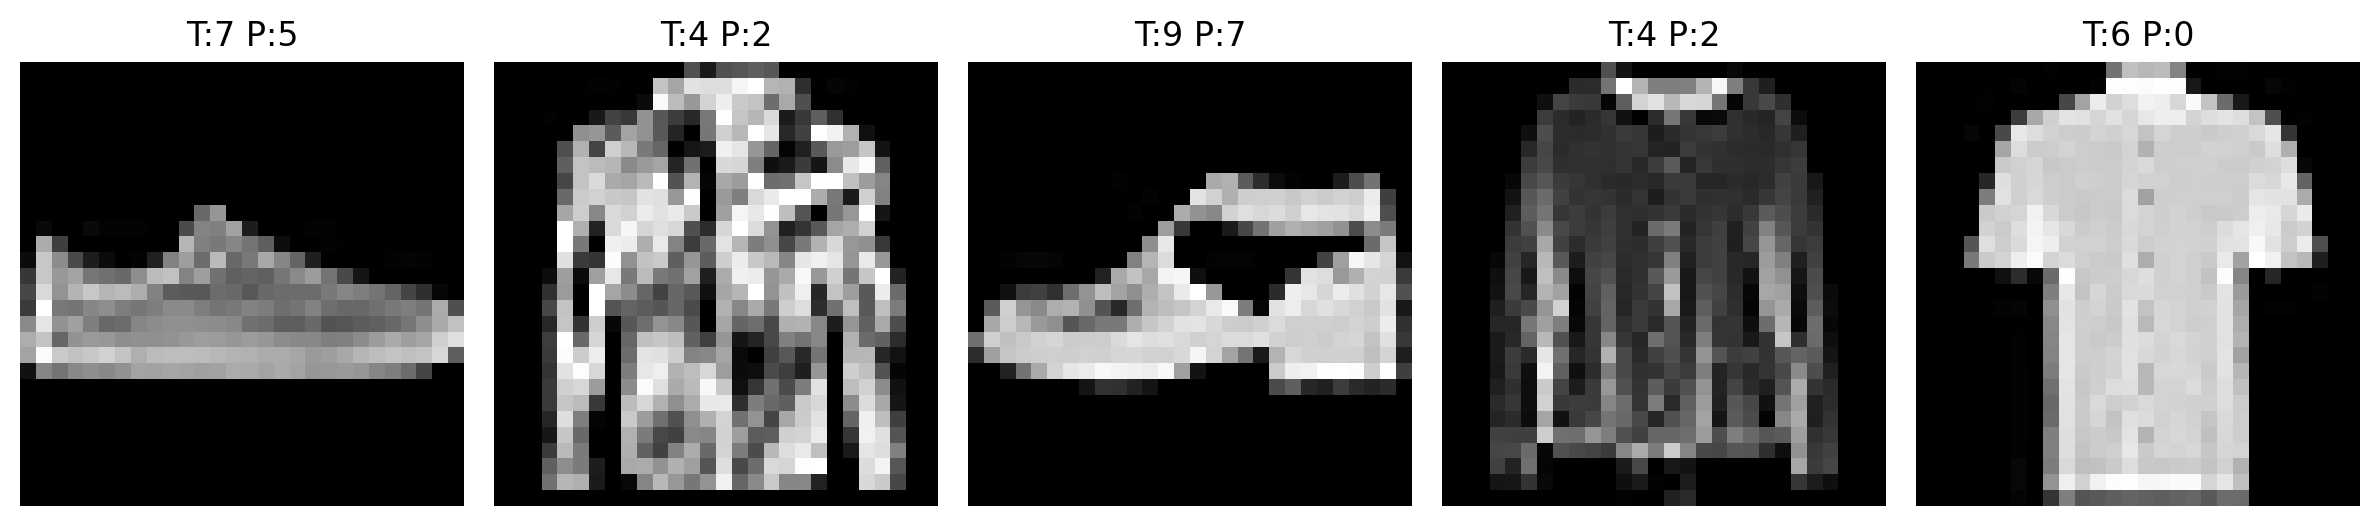
\includegraphics[width=\textwidth]{figures/question5/mlp_misclassified_examples.png}
\caption{Q5 MLP misclassified examples.}
\end{figure}

\begin{figure}[H]
\centering
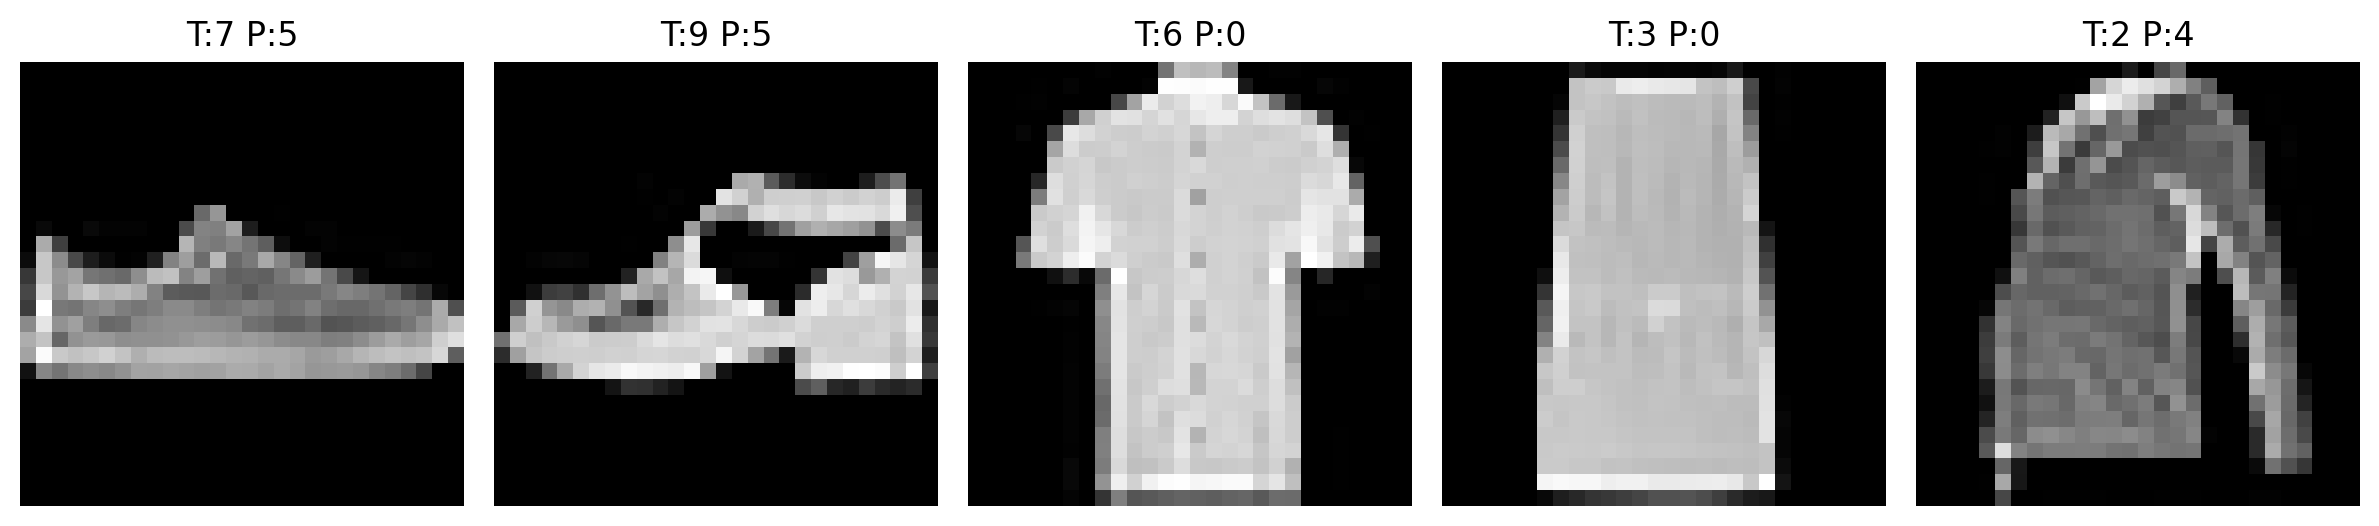
\includegraphics[width=\textwidth]{figures/question5/cnn_misclassified_examples.png}
\caption{Q5 CNN misclassified examples.}
\end{figure}

The most common confusions involved visually similar clothing categories such as shirts, T-shirts/tops, pullovers, and coats. The CNN still misclassified some borderline samples, but it generalized better overall because it preserved 2D structure throughout the feature extraction stage.

\section*{Conclusion}
Across all five questions, the consistent pattern was that model choice should follow data structure rather than popularity. Tree ensembles were strongest for nonlinear tabular regression, resampling materially changed minority-class recall in fraud detection, PCA balanced compression with downstream utility better than t-SNE, density-based clustering was highly parameter-sensitive, and CNNs outperformed MLPs once spatial information mattered.

\end{document}
